% interactcadsample.tex
% v1.03 - April 2017

\documentclass[]{interact}

\usepackage{epstopdf}% To incorporate .eps illustrations using PDFLaTeX, etc.
\usepackage{subfigure}% Support for small, `sub' figures and tables
%\usepackage[nolists,tablesfirst]{endfloat}% To `separate' figures and tables from text if required

\usepackage{anyfontsize}% allow to choose any font size in section
\usepackage{natbib}% Citation support using natbib.sty
\usepackage{booktabs} % For prettier tables
\usepackage{graphicx} % For prettier tables
\usepackage{caption,booktabs} % For prettier tables (center the label)

\usepackage{graphicx} % insert figure
\graphicspath{ {./figures/} }

\captionsetup{justification = centering}
\usepackage{hyperref} % linke table to text

\usepackage{har2nat} % Allows to use harvard package with natbib https://mirror.reismil.ch/CTAN/macros/latex/contrib/har2nat/har2nat.pdf

% For citing with natbib, you may want to use this reference sheet: 
% http://merkel.texture.rocks/Latex/natbib.php

\usepackage{setspace}

\usepackage{pdfpages} % we can include pdf figures into the article

\theoremstyle{plain}% Theorem-like structures provided by amsthm.sty

\newtheorem{theorem}{Theorem}[section]
\newtheorem{lemma}[theorem]{Lemma}
\newtheorem{corollary}[theorem]{Corollary}
\newtheorem{proposition}[theorem]{Proposition}

\theoremstyle{definition}
\newtheorem{definition}[theorem]{Definition}
\newtheorem{example}[theorem]{Example}

\theoremstyle{remark}
\newtheorem{remark}{Remark}
\newtheorem{notation}{Notation}

\begin{document}
	
	\begin{titlepage}
		\begin{center}
			\vspace*{0.3cm}
			
			\Huge
			\textbf{Changepoints Detection in Social Networks: an Extension of Relational Event Model}
			
			\vspace{1.8cm}
			\LARGE
			MID-TERM RESEARCH REPORT
			
			\vspace{1.8cm}
			
			\textbf{Hsuan Lee (9252568)}
			
			\vspace{1cm}
			Supervisors: 
			
			\vspace{0.5cm}
			
			Dr. Mahdi Shafiee Kamalabad 
			
			\& 
			
			Dr. Javier Garcia Bernardo
			
			\vspace{2cm}
			\Large
			
			\ Programme: MSBBSS
			
			\vspace{0.3cm}
			
			\emph{Department of Methodology \& Statistics}\\
			
			\vspace{0.3cm}
			Utrecht University\\
			the Netherlands\\
			
			\vspace{1.5cm}    
			\Large
			Date: 10.01.2023
			
			Words Count: 2497
			
			Candidate Journal: Social Networks
			
			FETC Case Number: 22-1870; 22-1871
		
		\end{center}
	\end{titlepage}
	
	\articletype{THESIS PROPOSAL}
	
	\vspace*{1cm}
	\hspace{-0.45cm}{\Large \textbf{Abstract}} \\

	Detecting changepoints is crucial in the social network field to identify the time points when stimulus occur in the network, providing insight into the dynamic evolution of the network. This paper presents an approach that facilitates the detection of changepoints in social networks by combining changepoint detection algorithms with the Moving Window-Relational Event Model (MW-REM). The MW-REM is a social network model that predicts future events and accounts for factors that influence social interactions. To capture the dynamics of the influence levels of these factors over time, the MW-REM uses the Moving Window (MW) approach that models each fitted window to capture fluctuations in the effects' influence level. The approach suggested in this paper incorporates changepoint detection algorithms to detect sudden shifts in the influence levels of these factors using the parameters given by the MW. Three competing changepoint detection algorithms (Binary Segmentation, Pruned Exact Linear Time, and Bayesian Online Changepoint Detection) are evaluated using synthetic data, and the best-performing algorithm is used to analyze real-life data. The approach can facilitate a better understanding of social dynamics, help identify potential challenges, and inform future strategies based on data. \\
	
	\hspace{-0.45cm}{\textbf{Keywords: }} \\
	{\small{Social network, Relational Event Model, Moving Window approach, Changepoints detection, Binary Segmentation, Pruned Exact Linear Time, Bayesian Online Changepoint Detection Method}
	
	\newpage


	\section{\fontsize{14}{15}\selectfont Introduction}
	
	\hspace{0.2cm} Changepoints are sudden shifts within the time series data which reflect the transitions occurring across conditions\cite{sharmaTrendAnalysisChange2016}\cite{aminikhanghahiSurveyMethodsTime2017}. The detection of changepoints is essential in many domains. In the social network area, due to the rich dynamics of social networks, changepoint detection allows us to spot the time points when certain stimulus occurred in the network, such as traffic accidents, organizational interventions, etc., assisting us to observe the dynamic evolution of the network more clearly. However, research and applications of changepoint detection are relatively lacking in the social network field.\\
	
	The aim of this study is to suggest an approach that facilitates detection of changepoints in social networks. To this end, we introduce changepoint detection methods into the structure of the relational event model (REM). The REM is a social network model that can predict the time and individuals involved in the future events in a social network. It is fitted in the relational event history (REH) data (\autoref{Table 1}), a social network data that at minimum contains information about the time, senders and receivers of events occurring in the social network. Generally, REM brings factors (e.g., gender, age, interaction inertia, etc.) that affect social interactions into the model through parameterization. Such factors are termed "effects"\cite{buttsRelationalEventFramework2008}, and the parameters of the REM represent the influence level of each effect in the social network. \\
	
	\begin{table}[h]
		\begin{tabular}{llll}
			\hline
			Time (hh,  mm, ss) & sender & receiver & message                                  \\ \hline
			13:14:05           & Patel  & Chen     & The weather conditions look good.        \\
			13:14:09           & Chen   & Patel    & Yes, it should be a smooth flight.       \\
			13:14:12           & Nguyen & Chen     & I've done my safety checks.              \\
			13:14:14           & Chen   & Nguyen   & Great job!                               \\ \hline
		\end{tabular}
	\caption{An Example of Relational Event History Data}
	\label{Table 1}
	\end{table}

	However, the influence level of effects in REM is assumed to hold constant over time, which seems unrealistic considering the dynamic nature of real-life interactions. To address this limitation, Mulder and Leenders \cite{mulderModelingEvolutionInteraction2019} proposed the Moving Window (MW) approach built upon the REM construct, which is capable of capturing the dynamics of the influence levels across time. The main concept of MW is to delineate specific duration of time (i.e. a window) that partially overlaps with the subsequent window and slides over the entire event history. Thereafter, by modeling each fitted window, we can model the fluctuations of the effects' influence level. The difficulty, however, is that the influence level typically varies between consecutive windows, leaving the visual identification of changepoints a challenge. \\
	
	In this study, we introduce changepoint detection algorithms (CPDs) into the combined MW-REM framework. By feeding these algorithms (influence level) parameters along the windows, we enable researchers to (1) infer a single specific changepoint at any given location, or (2) discover all changepoints across the REH. This can be employed on any social network scenario, such as: communication in the surgical room, interaction between teacher and students, as well as cooperation and competition between companies. The detection of changepoints can thus facilitate better understanding of social dynamics, help identify potential challenges as they appear and help inform future strategies based on data. In order to select the best CPD for MW-REM, three competing methods are presented and evaluated here: Binary Segmentation (BS), Pruned Exact Linear Time (PELT), and Bayesian Online Changepoint Detection (BOCPD). These methods will first be evaluated based on their Mean Squared Error (MSE), Confusion Matrix, and Mean Sign Difference (MSD) metrics, derived from synthetic data. Subsequently, the best-performing CPD will be additionally fitted on real-life data to test the method's external validity. The blueprint of the present study is shown in \autoref{Figure 1}. \\
	
	\begin{figure}[h]
		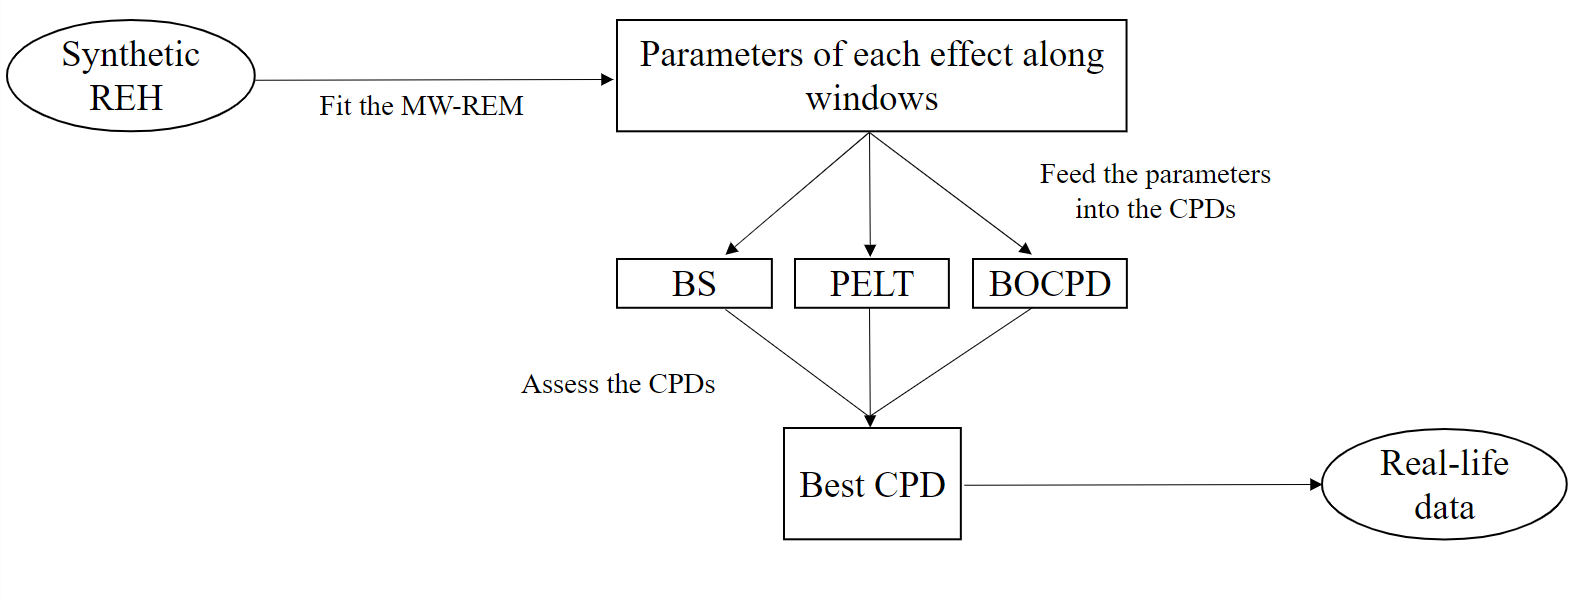
\includegraphics[width=14cm]{Flow_whole}
		\centering
		\caption{Flowchart Depicting the Research Design of the Present Study}
		\label{Figure 1}
	\end{figure}
	
	\section{\fontsize{14}{15}\selectfont Theoretical Background}
	
	\subsection{Relational Event Model (REM)}
	
	\hspace{0.2cm} The model relied on in this study is REM, proposed by Butts\cite{buttsRelationalEventFramework2008}. By fitting the REM, the influence level of certain effects on entire social networks becomes observable, the information about the next event as well is predictable. This facilitates the manipulation of changepoint detection methods.\\ 
	
	REM builds models on network data that have sender, receiver and time information, denoted as (s,r,t), which are referred to as Relational Event History Data (REH)\ref{Table 1}. The main attribute of REM is that it parameterizes the effects. Typically, effects can be categorized into exogenous and endogenous variables. Exogenous variables are features belonging to actors which are not derived from past interactions between actors in the REH, but still influence the development of social interactions, e.g., gender, age, etc. Endogenous variables are specific effects derived from given properties of past interactions between actors in the REH, e.g., inertia, transitivity, etc.\\
	
	In REM, each combination of actors, i.e., $(s,r)$, has the possibility of occurring at time $t$ of each event, these potential sender-receiver pairs at time $t$ is termed risk set, denoted as $R(t)$. The size of risk set of an event is typically $N \times (N-1)$, where $N$ represents the number of actors in the social network, as each actor can be either a sender or a receiver, but not both a sender and a receiver. The REM is virtually modeling the event rate($\lambda$) that predict which sender-receiver pair $(s,r)$ will be involved in the next event and when it will occur, i.e., each $(s,r)$ pair is equipped with its own event rate for each event and is assumed to stay invariant between the time of the present event and the time of the following event. As a rule, the $(s,r)$ pair with a higher event rate in the risk set R at time t is more probable to occur in the next event, and the probability of the $(s,r)$ pair taking place in the next event follows a multinomial distribution:
	\begin{equation} \label{1}
		P \left((s,r) | t \right) = \dfrac{\lambda(s,r,t)} {\sum_{R(t)} \lambda(s,r,t)}
	\end{equation}
	, where $\lambda(s,r,t)$ represents the event rate of a pair (s,r), $R(t)$ denotes the risk set for time $t$. \\
	
	On the other hand, the duration between the two events follows an exponential distribution: 
	\begin{equation} \label{2}
		\Delta t \sim Exponential \left(\sum_{R(t)} \lambda(s,r,t) \right)
	\end{equation}
	, where $\Delta t$ implies the duration between two events; the higher the total event rate of the risk set, the shorter the $\Delta t$. \\
	
	In terms of the event rate, it is typically considered as a log-linear function of the outcome in REM with specific effects:
	\begin{equation} \label{3}
		\log \lambda(s,r,t) = \sum_{p} \beta_p x_p(s,r,t)
	\end{equation}
	, where $\beta_p$ represents the parameter of effects, which expresses the influence level of one effect on the entire social network; $x_p(s,r,t)$ denotes the statistics, which can be either an exogenous or endogenous variable. \\
	
	By modeling the event rate, the time and actors of the next event can be predicted; a major weakness of REM, however, is that it assumes that the influence level of effects are constant over the event history (i.e., $\beta_p$), which is impractical given the dynamic character of social interactions.
	
	\subsection{Moving Window Approach (MW)}
	
	\hspace{0.2cm} To get rid of the above mentioned limitations of REM, Mulder and Leenders proposed the Moving Window approach(MW) under REM structure in 2019\cite{mulderModelingEvolutionInteraction2019}. The basic thought of the MW approach is to setup a fixed size window, i.e. a fixed length of time, sliding over the entire REH, with each window sharing a fixed size overlap with the previous one, then fitting the REM on each window (\autoref{Figure 1}). This way, the influence level of each effect on the social network along time is revealed by the parameters given in each window. As such, the thought of this study is to execute the changepoint detection algorithms on the given parameters in each window of the entire REH. \\ 
	
	An advantage of the MW approach is that it unveils the dynamics of the social network across time, which is beyond the reach of the original REM. But a point to note about the MW approach is that each window possesses a different number of occurred events, those with too few events can result in bias, as well as instability of the parameters of the windows\cite{mulderModelingEvolutionInteraction2019}, thus, it is crucial to choose a decent window size and overlap. \\
	
	The shortcoming of the MW approach is that the window size and overlap are fixed, coupled with its aggregation feature, which in certain scenarios can hide the event that the parameters shift rapidly at particular time points. To address this downside of the MW approach, the Data-Driven Moving Window approach (DDMW) was proposed by Meijerink-Bosman \cite{meijerink-bosmanDynamicRelationalEvent2022}, which allows the window size to vary along the observed event history, with larger windows for events that do not carry sharp changes in parameters; smaller windows for events with drastic shifts in parameters. The window size variation mechanism of DDMW is based on the Bayes Factor (BF), which enables to quantify the relative support of two hypotheses in the data by the ratio of two marginal likelihoods \cite{guApproximatedAdjustedFractional2018}. \\
	
	DDMW starts with the researcher proposing a minimum window size in which the duration is equally separated by i partitions (again selected by the researcher), followed by BF assessing the relative support for the "hypothesis that the effect within the window size range is static" against the "hypothesis that the effect within the window size range is dynamic" by parameter changes along the i partitions, the two hypotheses are expressed as:
	\begin{gather} \label{4, 5}
		H_{static}: \beta_1... = \beta_i... = \beta_I \\ 
		H_{dynamic}: not\hspace{0.15cm} H_{static}
	\end{gather} 
	, where $\beta$ represents the parameter(influence level) of a effect, I denotes the number of partitions within a window.\\
	
	Owing to the prior sensitivity of BF, DDMW uses "multiple population adjusted approximate fractional Bayes Factors", which allows automatic computation of the prior without any prior beliefs. The BF of DDMW builds an implicit default prior by taking a fraction $p_i$ of the likelihood information for each partition i, expressed as\cite{hoijtinkBayesianEvaluationInformative2019}:
	\begin{equation} \label{6}
		p_i = \dfrac{1}{I} \times J^* \times \dfrac{1}{N_i}
	\end{equation}
	, where $i$ represents the partition $i$ in the window, $J^*$ denotes the number of independent constraints from $H_{static}$(i.e., $J^* = I - 1$), $N_i$ implies the number of events in partition $i$. The relative support of $H_{static}$ and $H_{dynamic}$ in the data is the ratio of the fit and complexity of $H_{static}$ versus $H_{dynamic}$, which is quantified as\cite{meijerink-bosmanDynamicRelationalEvent2022}: 
	\begin{equation} \label{7}
		BF = \dfrac{\int_{\beta \in H_{static}} \mathcal{N}(\beta|\hat{\beta}, \hat{\sum}_{\beta}) d\beta}
		{\int_{\beta \in H_{static}} \mathcal{N}(\beta|\beta_P, \hat{\sum} ^p _{\beta}) d\beta}
	\end{equation}
	, where $\beta$ denotes the set of i parameters of the window, i.e., $\beta_1, \beta_2... , \beta_i$, $\hat{\beta}$ represents an estimate of the maximum likelihood of $\beta$, $\hat{\sum}_\beta$ indicates the corresponding covariance matrix, $\beta_P$ implies the adjusted mean of the prior distribution, which is 0 in the DDMW, $\hat{\sum} ^p _\beta$ expresses the covariance matrix of the prior distribution of $\beta$, based on information from a fraction $p$ of the data.\\
	
	Due to the property of BF, if BF equals $K$, it implies that one hypothesis has $K$ times more statistical evidence than the other. That is, if the BF in DDMW is greater than 0, the data prefers the static hypothesis. Thus, in the DDMW setup, if $\log$ BF is greater than 0, the window size is iteratively increased so that more events enter the window until $\log\dfrac{1}{10}$ (the BF is calculated with $I$ = 3). \\
	
	However, albeit DDMW is considered more precise than MW, it is relatively more computationally expensive. In this study, MW is adopted for synthetic data, as we have a clearer and more comprehensive picture of it; whereas DDMW is employed for real-life data. \\
	
	\begin{figure}[h]
		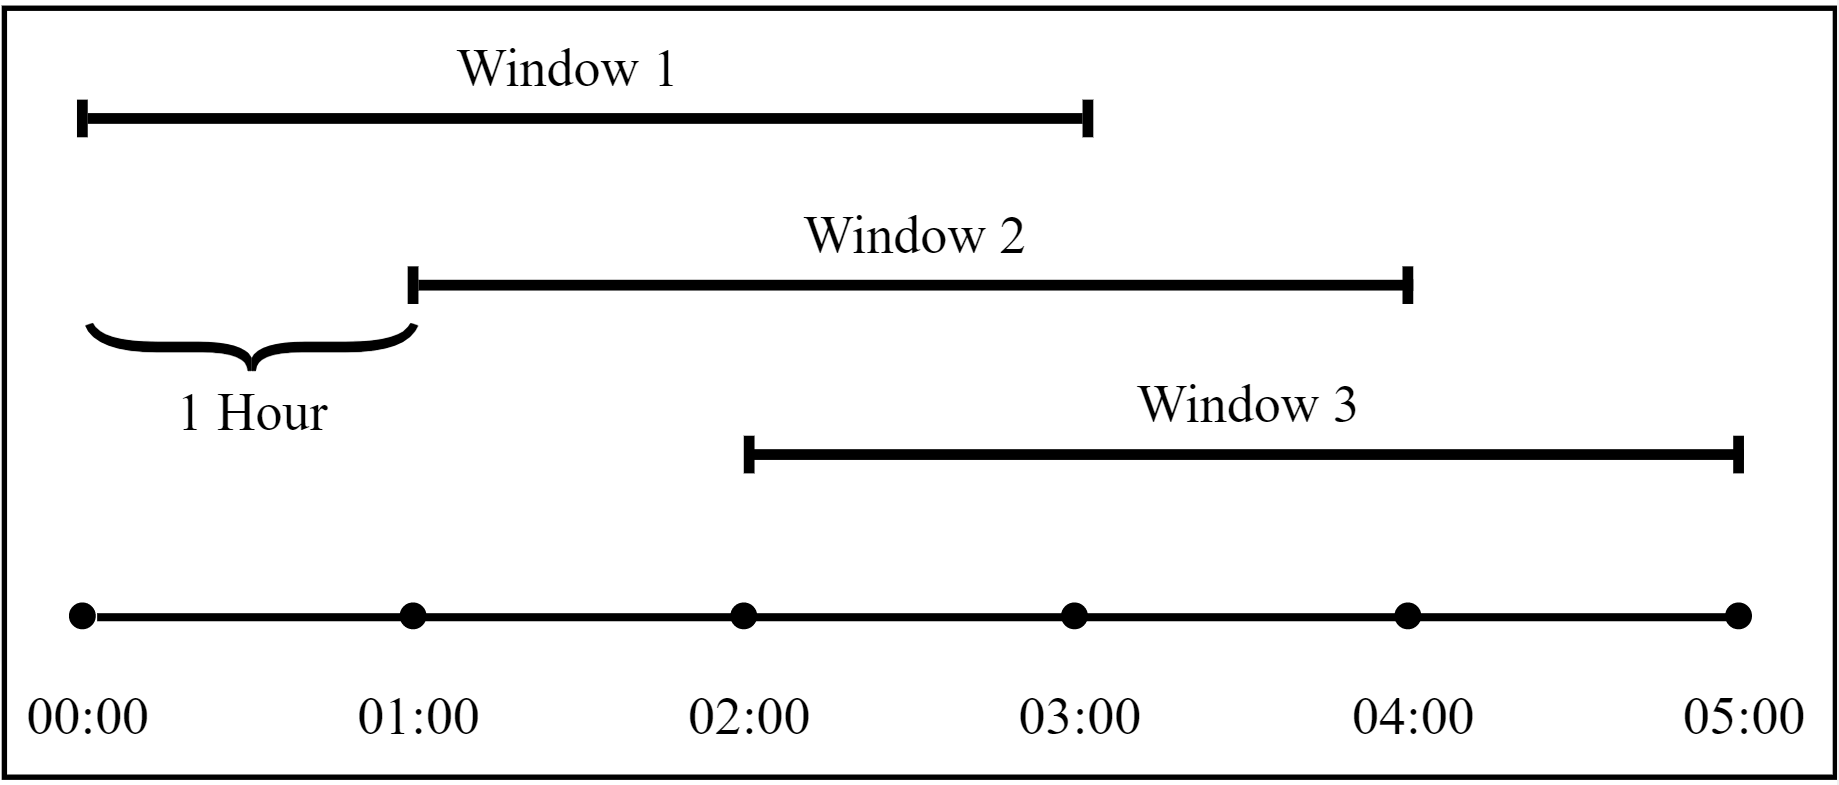
\includegraphics[width=13cm]{MW}
		\centering
		\caption{An Example of Moving Window Approach}
		\label{Figure 2}
	\end{figure}
	
	\subsection{Changepoint Detection Methods (CPDs)}
	
	\hspace{0.2cm} The importance of applying changepoint detection in REH stems from the fact that important evolution of effects in social networks across time become identifiable, via this, one can somehow prevent unexpected emergencies or better cope with upcoming issues. Regarding relevant studies on inferring CPs in REH, Shafiee Kamalabad suggested inferring changepoints in social networks by Bayes Factor, which uses the support of two hypotheses from the data to prove the existence of changepoints \cite{kamalabadWhatPointChange}. Apart from this study, however, CPD studies for REH are still comparatively rare. \\
	
	Typically, CPDs are classified into two categories, i.e. online methods and offline methods. Online methods, which aim to detect changes immediately in a real-time context; Offline methods, which intend to examine changes retrospectively upon collection of complete data \cite{truongSelectiveReviewOffline2020}. In this study, an offline method, i.e., Binary Segmentation, is introduced; and two online methods, i.e., PELT and BOCPD, are presented. \\
	
	\hspace{-0.55cm} \textbf{Binary Segmentation (BS)}\\
	
	BS is the most commonly used CPD in many research areas. BS recognizes the changepoints by computing the time point in the data that minimizes the given cost function, then divides the data into two segments by it(i.e., the location of the changepoint), after which the same procedures are performed in each separated sub-segment until no changepoint is left in each segment \cite{killickOptimalDetectionChangepoints2012}. \\
	
	In changepoint detection, the cost function is a quality measure that splits the data into segments. CPD is designed to segment the data at the time point where the cost function is minimized. The most common cost function for multiple changepoint detection is \cite{killickOptimalDetectionChangepoints2012}:
	\begin{equation} \label{8}
		\sum_{i = 1} ^{m + 1} \left[C(y_{({\tau_{i-1} + 1}):\tau_{i}}) \right] + \beta f(m)
	\end{equation}
	, where $i$ denotes the order of a time point in a segment, $m$ indicates the number of changepoints, $\tau_i$ implies the location of a possible changepoint (i.e., time point $i$). And the m changepoints will divide the data into $m+1$ segments, with the $i$th segment contains $y_{({\tau_{i-1} + 1}):\tau_{i}}$. $C$ represents the cost function of a segment, $\beta f(m)$ serves as a penalty to prevent overfitting. \\
	
	For BS, the recognized changepoints of the data are required to meet the criteria:
	\begin{equation} \label{9}
		C(y_{1:\tau}) + C(y_{({\tau + 1}):n}) + \beta < C(y_{1:n})
	\end{equation}
	BS continues to search for possible changepoints until there is no $\tau$ that meets the criteria, then BS stops. \\
	
	\hspace{-0.55cm} \textbf{Pruned Exact Linear Time (PELT)}\\
	
	The PELT is a method based on the Segment Neighborhood changepoint detection method (SN)\cite{augerAlgorithmsOptimalIdentification1989}. SN employs dynamic programming to scan the entire segmented area. It first establishes the maximum number of changepoints, next evaluates the cost function of all possible segments. Eventually, the number of changepoints of the data is between 0 and the previously set maximum number. Further, the SN is capable of including any form of penalty(i.e., $\beta f(m)$), yet with the drawback of high computational cost. \\
	
	The PELT solves the high computational cost of SN whilst maintaining the accuracy of identifying changepoints. It improves computational efficiency by removing the value of $\tau$ from each iteration that is unlikely to be the minimum value, simultaneously searching for the value of $\tau$ that minimizes the cost function below \cite{killickOptimalDetectionChangepoints2012}:
	\begin{equation} \label{10}
		\sum_{i = 1} ^{m + 1} \left[C(y_{({\tau_{i-1} + 1}):\tau_{i}}) + \beta \right]
	\end{equation}
	, which is equivalent to \eqref{8}, where $f(m)$ = $m$. The PELT considers the cost function of all potential segments, which ranges between 0 and the previously set maximum number of changepoints, and stops when no more changepoints are detected.\\
	
	\hspace{-0.55cm} \textbf{Bayesian Online Changepoint Detection (BOCPD)}\\
	
	Unlike BS and PELT, which rely on cost functions to identify changepoints, BOCPD infers changepoints based on Bayesian approach, which define changepoints in terms of posterior probabilities (i.e., run length probabilities) at time points. \\
	
	In BOCPD, run length is an essential concept, it represents the length of time points elapsed since the last identified changepoint, which can be understood as akin to the segments in PELT and BS. Whenever BOCPD recognizes a changepoint, the run length drops to 0 and recalculates the length. To determine the changepoints, BOCPD is required to calculate the run length probabilities (i.e., posterior probabilities) for each time point. Given that each time point contains probabilities of increase and decrease in run length, the run length probabilities thus includes both growth probabilities and changepoint probabilities. According to Adams and Mackay\cite{adamsBayesianOnlineChangepoint2007}, to save computational costs, it is suggested to set a cut-off point for the run length probability, typically $10^{-4}$, where if the run length probability reaches such cut-off point, the time point is determined as a changepoint. \\
	
	Overall, the BOCPD starts by building the predictive distribution from the potential locations of changepoints, which reveals any prior knowledge regarding the data generation process. Then, based on the given predictive distribution, the BOCPD computes the run length probability at a time point, with new data coming in, the predictive distribution is continuously updated, the BOCPD iteratively runs the same procedure until no new data appear. \\
	
	\section{\fontsize{14}{15}\selectfont Methodology}
	
	\hspace{0.2cm} This study relies on two types of data: synthetic and real-life data; the real-life data is the Apollo 13 voice-loop data publicly available from NASA, both datasets have passed ethical consent. All the analyses on this research are performed by R. The package "remstats" is used to simulate the REH to test the performance of CPDs in different scenarios; the package "relevent" is designed to fit the REM to the REH. Additionally, package "changepoint" is employed to apply CPs detection methods, such as BS, PELT; package "ocp" is adopted to operate BOCPD. For other side, package "tidyverse" is assigned for data cleaning and visualization work.\\
	
	\hspace{-0.55cm} \textbf{Phase 1 - data generation}\\
	
	Ten synthetic REH datasets are generated based on the MW-REM, These datasets are designed to involve four effects with two exogenous and two endogenous variables, the exogenous variables are: " Sender effect", which refers to exogenous actor attributes that influence the actor's rate of sending events; "Difference", which signifies the difference in actor personal attributes that affect the rate of sending events; the endogenous variables are:" Inertia," which was defined as the tendency of actors to repeatedly select the same actor as the receiver of their events; and "Outdegree of the Sender effect", which expresses the tendency of actors to send events if they have sent more events in the past. \\
	
	In the 10 synthetic datasets, one is purposed to have no changepoint in the entire REH for each effect; three are set to have one changepoint across the REH; three are targeted to have two changepoints throughout the REH; and three are designed to have three changepoints across the REH. For the datasets with changepoints, three scenarios are created (\autoref{Table 2}), one with only inertia having changepoint(s) while the remaining effects have no changepoint; one with the changepoint(s) for each effect at the same location of the window(s); and one with the changepoint(s) for each effect at different locations of the window(s). \\
	
	\begin{table}[h]
		\centering
		\small
		\begin{tabular}{|l|c|c|}
			\hline
			\textbf{No. of CPs} & \multicolumn{1}{l|}{\textbf{CPs Location}} & \multicolumn{1}{l|}{\textbf{Effects with CPs}} \\ \hline
			0 Changepoint                &                                                                &                \\ \hline
			&                                                                & Inertia                                     \\ \cline{2-3} 
			1 Changepoint                & Same Window                                                    & All                                    \\ \cline{2-3} 
			& Different Windows                                              & All                                         \\ \hline
			&                                                                & Inertia                                     \\ \cline{2-3} 
			2 Changepoints               & Same Windows                                                   & All                                    \\ \cline{2-3} 
			& Different Windows                                              & All                                         \\ \hline
			&                                                                & Inertia                                     \\ \cline{2-3} 
			3 Changepoints               & Same Windows                                                   & All                                    \\ \cline{2-3} 
			& Different Windows                                              & All                                         \\ \hline
		\end{tabular}
		\caption{Synthetic REH Dataset, where CP refers to changepoint.}
		\label{Table 2}
	\end{table}
	
	\hspace{-0.55cm} \textbf{Phase 2 - the CPD's performance and comparison}\\
	
	The MW-REM are fitted to the synthetic datasets, followed by performing the BS, PELT and BOCPD on the parameters given by the windows (the influence level of the effects over time). Thereafter, to examine the feasibility, the confusion matrix is utilized, which allows us to determine if a CPD is capable of detecting the correct number of changepoints; and to compare the performance \cite{aminikhanghahiSurveyMethodsTime2017}, the Mean Squared Error (MSE) is employed,  expressed as:
	\begin{equation} \label{11}
		MSE = \frac{\sum_{i = 1}^{\#CP} (Predicted(CP) - Actual(CP))^2}{\#CP}
	\end{equation}
	, where $CP$ denotes the changepoint, $\#CP$ represents the number of changepoints. The MSE quantifies the accuracy of CPD, the lower the MSE, the higher precision of CPD. In this study, MSE is measured for all ten synthetic datasets, and the average of MSE for each CPD is considered, from which it is possible to know which of the three CPDs offers the best performance under the MW-REM structure. \\
	
	On the other hand, each CPD has its own custom of identifying changepoints, i.e., tending to infer changepoints ahead of or behind the true changepoints. To assess the habit of each CPD in the REH construct, Mean Signed Difference(MSD) is adopted, expressed as \cite{aminikhanghahiSurveyMethodsTime2017}:
	\begin{equation} \label{12}
		MSD = \frac{\sum_{i = 1}^{\#CP} (Predicted(CP) - Actual(CP))}{\#CP}
	\end{equation}
	MSD considers the direction of the error. With a negative MSD, CPD prefers to predict the changepoints before the true changepoints; with a positive MSD, CPD prefers to predict the changepoints after the real changepoints. In this study, MSD for all ten synthetic datasets are measured, the average value of MSD for each CPD is regarded, from which the custom of each CPD under the MW-REM structure becomes observable. \\
	
	Totally, we will conclude which CPD possesses the best accuracy under the REH construct by MSE, together with the proper application scenarios for each CPD based on MSD. Eventually, the CPD with the best accuracy will be adopted for the real-life data. \\
	
	\hspace{-0.55cm} \textbf{Phase 3 - performing on real-life REH data}\\
	
	The real-life data utilized in this study is the Apollo 13 voice loop data publicly available from NASA.\\
	
	Apollo 13 was a failed mission in the Apollo space program aimed at landing on the Moon. The failure of it was triggered by a routine agitation of one of the oxygen tanks that ignited the damaged wire insulation inside, resulting in an explosion that discharged the contents of both SM's oxygen tanks into space, thereby leaving the astronauts without systems to generate electricity and oxygen. To address the emergency, the astronauts contacted Mission Control to help them manage the issues, and the mission was canceled. \\
	
	In the Apollo 13 voice loop data, there was a time point that an astronaut said, "Houston, we've had a problem here." With this, we are able to establish that that was the time when the emergency occurred, that is, the location of the changepoint. To test the performance of CPD in practice, the DDMW-REM is fitted on the Apollo 13 voice loop data, as DDMW shows better performance on the actual data compared to the original MW, then the CPD with the best accuracy from synthetic data is manipulated on the parameters given by the windows.\\
	
	The purpose of this phase is to examine whether the CPD with the best accuracy from synthetic data also functions properly in real life, i.e., detecting the changepoint near the actual one from Apollo 13 voice loop data. In summary, If CPD performs well in the Apollo 13 voice loop data, it can be concluded that CPD is available to be introduced into the REM structure and succeeds in recognizing changepoints in a social network, conversely, if CPD fails to work properly, the changepoints in a social network may have to be inferred by other means. \\
	
	\newpage
	
	\nocite{*} % Print all the References out, not only the citing
	\bibliographystyle{abbrv}
	\bibliography{My_Library}
	
\end{document}
